% Preamble:
\documentclass{article}

% Packages:
\usepackage{fancyhdr}
\usepackage{amsmath}
\usepackage{graphicx}
\usepackage{mathbbol}
\usepackage{tikz}
\usetikzlibrary{arrows}
\usetikzlibrary{backgrounds}

% Title Page Information:
\title{CS23 Assignment Five}
\author{CJ Bridgman-Ford \\ cj.ikaika@gmail.com}
\date{April 16, 2024}

% Make subsections lettered:
\renewcommand{\thesubsection}{\alph{subsection}.}

% fancyhdr Page Styling:
\newcommand{\pagenumber}{\thepage\quad}
\newcommand{\authorname}{CJ Bridgman-Ford}

\pagestyle{fancy}
\renewcommand{\headrulewidth}{0pt}
\fancyhead{}
\fancyfoot[L]{\authorname}
\fancyfoot[C]{}
\fancyfoot[R]{\pagenumber}

% End of Preamble.

% Start of document:
\begin{document}

% Title Page:
\maketitle
\thispagestyle{empty}

\clearpage
% Page 1:
\pagenumbering{arabic}

% Problem 1:

\section{If 12 people shake hands with each other, how many
    handshakes take place.}
\hspace{1cm}\textit{In order to solve this problem, we are
    looking for how many ways we can create groups of $2$
    people from the $12$. This leads us to the combinations
    formula: $nCr$, where $n$ is the total number of people
    and $r$ represents a single handshake between $2$ people.
    See below:}
\begin{center}
    \large{$nCr = C(n,r) = \frac{n!}{r!(n-r)!}$}
    \large{$\xrightarrow{} C(12,2) = \frac{12!}{2!(12-2)!}
        = 66$.} \\
\end{center}
\hspace{1cm}\textit{Thus, $66$ handshakes take place.}

% Problem 2

\section{In a group of six people, is it possible for everyone
    to be friends with exactly two other people in the group?
    How about three other people? Four?}
\hspace{1cm}\textit{While drawing out graphs is an option, an
    easier and more straightforward approach involves counting
    the number of degrees between each node. The sum of degrees
    must be always be even because it takes two nodes to form
    an edge. Let's apply this logic to the question. If each person
    is repesented by a node, and each friendship by an edge, then the
    number of degrees on each node is the number of friends any given
    person has. Thus, we can evaluate the boolean of the following
    statement see if each case is possible:}
\begin{center}
    \large{True or false: For $n$ nodes, each with $r$ degrees, is 
    $\frac{n\cdot r}{2} \in \mathbb{Z}$?} \\
    \vspace{0.25cm}
    \normalsize{}
    \begin{tabular}{|c|c|c|c|}
        \hline
        Number of People & Number of Friends & Statement & True or False \\
        \hline
        6 & 2 & $(6\cdot 2)/2 = 6$ & True \\
        6 & 3 & $(6\cdot 3)/2 = 9$ & True \\
        6 & 4 & $(6\cdot 4)/2 = 12$ & True \\
        \hline
    \end{tabular}
\end{center}
\hspace{1cm}\textit{Thus, we can see that each combination of number
    of friends is possible.}
\clearpage

% Problem 3:

\section{Is it possible for two graphs with the same number of nodes
    and edges to not be isomorphic? What if the degrees of the nodes in
    the two graphs are the same? Give example graphs or explain why.}
\hspace{1cm}\textit{Take a look at the graphs below. They each have $6$
    nodes and $9$ edges, yet are not isomorphic. While the sum of
    all node degrees in both graphs is $18$, the bipartite graph's nodes
    are evenly distributed, whereas its opposition's are not. Therefore, 
    if the node degrees differ, non-isomorphic graphs are clearly possible.}
\begin{center}
    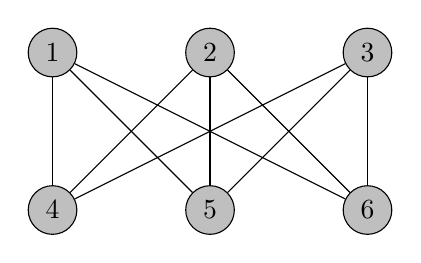
\begin{tikzpicture}
        \node[draw, circle, fill=gray!50] (node1) at (0,2) {1};  
        \node[draw, circle, fill=gray!50] (node2) at (2,2) {2};  
        \node[draw, circle, fill=gray!50] (node3) at (4,2) {3};  
        \node[draw, circle, fill=gray!50] (node4) at (0,0) {4};  
        \node[draw, circle, fill=gray!50] (node5) at (2,0) {5};  
        \node[draw, circle, fill=gray!50] (node6) at (4,0) {6};
        
        \draw (node1) -- (node4);
        \draw (node1) -- (node5);
        \draw (node1) -- (node6);
        \draw (node2) -- (node4);
        \draw (node2) -- (node5);
        \draw (node2) -- (node6);
        \draw (node3) -- (node4);
        \draw (node3) -- (node5);
        \draw (node3) -- (node6);
    \end{tikzpicture} \\
    \vspace{0.5cm}
    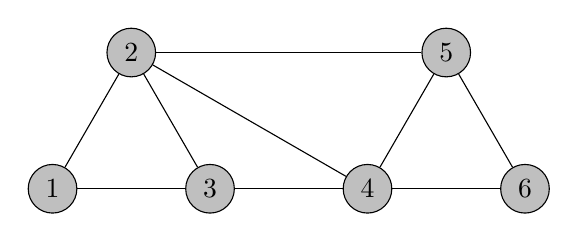
\begin{tikzpicture}
        \node[draw, circle, fill=gray!50] (node1) at (0,0) {1};  
        \node[draw, circle, fill=gray!50] (node2) at (1,1.73) {2};  
        \node[draw, circle, fill=gray!50] (node3) at (2,0) {3};  
        \node[draw, circle, fill=gray!50] (node4) at (4,0) {4};  
        \node[draw, circle, fill=gray!50] (node5) at (5,1.73) {5};  
        \node[draw, circle, fill=gray!50] (node6) at (6,0) {6};
        
        \draw (node1) -- (node2);
        \draw (node1) -- (node3);
        \draw (node2) -- (node3);
        \draw (node4) -- (node5);
        \draw (node4) -- (node6);
        \draw (node5) -- (node6);
        \draw (node2) -- (node5);
        \draw (node3) -- (node4);
        \draw (node2) -- (node4);
    \end{tikzpicture} \\
\end{center}
\vspace{0.25cm}
\hspace{1cm}\textit{But what if all the nodes have the same degree? In that case,
    every graph with the same number of nodes and edges would be isomophic. (Note:
    this logic requires the graph to be nondirectional. If the connections between
    nodes indicate or carry direction, then you could still find ways to create two
    or more non-isomophic graphs.)}
\clearpage

% Problem 4:

\section{What is the largest number of edges possible in a graph with 10 vertices?
    What is the largest number of edges possible in a bipartite graph with 10 vertices?
    What is the largest number of edges possible in a tree with 10 vertices?}
\hspace{1cm}\textit{The first portion of this question is nearly identical in logic to 
    Problem 1. The maximum number of edges possible in a graph with 10 vertices would occur
    where each vertex connects to each and every other vertex; Every person shakes
    hands with each and every other person. Thus:}
\begin{center}
    \large{$nCr = C(n,r) = \frac{n!}{r!(n-r)!}$}
    \large{$\xrightarrow{} C(10,2) = \frac{10!}{2!(10-2)!}
        = 45$ edges.} \\
\end{center}
\hspace{1cm}\textit{What about in a bipartite graph? In a bipartite graph, edges are formed
    between two distinct sets of
    vertices. Thus, we can count the node degrees in either
    set, sum them up, and that will give us our edges. If $V$ is our number of vertices, 
    we can form, at most, $V/2$ connections per node, and still have a bipartite graph.
    If we sum up this max per every node in either (but not both) set(s), we would sum the node
    degrees $V/2$ times. Thus, our equation becomes $(V/2)^2$. (Note: This calculation assumes
    that $V$ is an even number.)}
\begin{center}
    \large{$(\frac{V}{2})^2 \xrightarrow{} (\frac{10}{2})^2 = 25$ edges.} \\
\end{center}
\hspace{1cm}\textit{What about in a tree graph? One of the characterizing traits of tree graphs is that 
they do not contain cycles. In a tree graph, there will always be $(V-1)$ edges, where $V$ is
the number of vertices. Therefore:}
\begin{center}
    \large{$(V-1) \xrightarrow{} (10-1) = 9$ edges.} \\
\end{center}
\clearpage

% Problem 5:

\section{Consider graphs with $n$ vertices. Remember, graphs do not need to be connected.}
\subsection{How many edges must the graph have to guarantee at least one vertex has degree
    two or more? Prove your answer.}
\hspace{1cm}\textit{Imagine $3$ vertices in a triangular pattern. We can start by adding one
    edge, which means two vertices will have a degree of $1$. Next, we'll add another edge. It
    is at this point (2 edges) that at least one vertex will have a degree of $2$. Repeat this process for
    $4$ vertices in a square (3 edges), $5$ vertices in a pentagon (3 edges), and $6$ vertices in
    a hexagon (4 edges). At this point, the pattern has emerged. Let's define a function $L_{2\mathbb{Z}}(n)$,
    that rounds down to the nearest even integer. By analyzing this pattern, we see that the number of edges
    will be $\frac{L_{2\mathbb{Z}}(n)}{2}+1$. This is because, for all the vertices in a graph to be of degree $1$,
    $n$ must be even such that the nodes can become isolated pairs with single edges. At this point, the number of
    vertices would be $n/2$. Adding an extra edge would cause one of the nodes to raise in degree.}
\subsection{How many edges must the graph have to guarantee all vertices have a degree of
    two or more? Prove your answer.}
\hspace{1cm}\textit{Let's return to our logic from part a and run through the scenarios once again,
    counting how many edges we need before our new criteria is met. For a triangle, it's $3$ edges,
    a square, $4$, a pentagon, $5$...so on and so forth. This one is simpler to prove, as all of the
    node degrees in a graph must sum to an even number. Which, when divided in half, returns the number
    of edges in the graph. So, if you have $n$ vertices, and they all must have a degree of $D$, then the
    number of edges would be equal to $\frac{n\cdot D}{2}$. Solving this for $D=2$, we get $\frac{n\cdot 2}{2} = n$.}
\clearpage

% Problem 6:

\section{Refer to the figure below:}
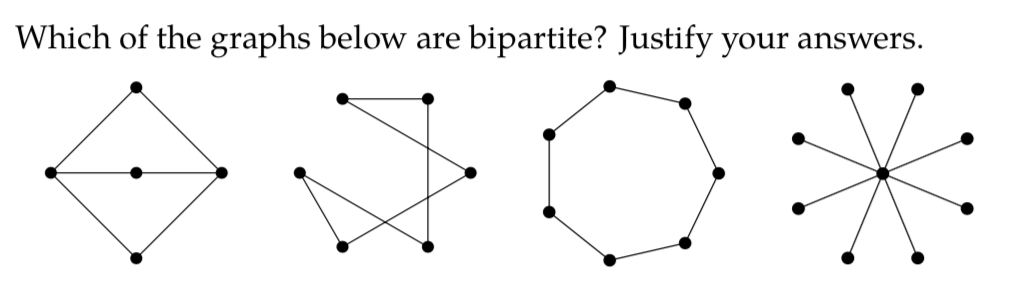
\includegraphics[scale=0.66]{assignment5-problem6.png}

\hspace{1cm}\textit{Starting from the left, let's call these graphs A, B, C, and D. Every graph, except for C, is bipartite.}
\subsection{Graph A: Visual Proof.}
\begin{center}
    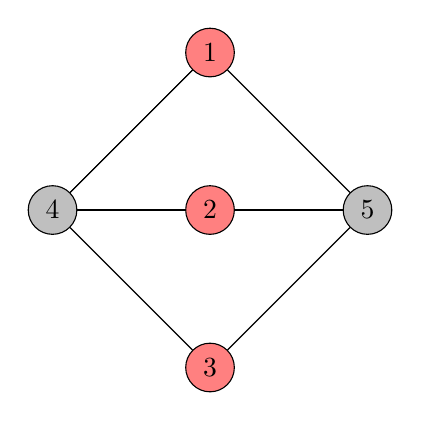
\begin{tikzpicture}
        \node[draw, circle, fill=red!50] (node1) at (0,2) {1};  
        \node[draw, circle, fill=red!50] (node2) at (0,0) {2};  
        \node[draw, circle, fill=red!50] (node3) at (0,-2) {3}; 
        \node[draw, circle, fill=gray!50] (node4) at (-2,0) {4};  
        \node[draw, circle, fill=gray!50] (node5) at (2,0) {5};  
        \draw (node1) -- (node4);
        \draw (node1) -- (node5);
        \draw (node2) -- (node4);
        \draw (node2) -- (node5);
        \draw (node1) -- (node4);
        \draw (node3) -- (node4);
        \draw (node3) -- (node5);
    \end{tikzpicture}
\end{center}

\subsection{Graph B: Written Explanation}
\hspace{1cm}\textit{Since Graph B has an even number of nodes and a cyclical 
    strcuture, by assigning sets in an alternating pattern (Node 1 $\in$ Set A,
    Node 2 $\in$ Set B, Node 3 $\in$ set A, etc), we identify that the graph is
    bipartite.}
\subsection{Graph C: Written Explanation}
\hspace{1cm}\textit{Graph C has the same cyclical structure as Graph B, meaning
    that we would apply the same logic. However, since Graph C has an odd number
    of nodes, there is no way to divide up the nodes into two distinct sets that 
    form a bipartite graph.}
\subsection{Graph D: Written Explanation}
\hspace{1cm}\textit{Graph D can be proven to be bipartite by assigning the center
    node to Set A, and the orbiting nodes to Set B.}

\end{document}